\begin{exsol}{21}{\MR{} Analytical Problem 5.4}{165}{Exam}{B3}
\asked A used-car seller and a buyer each hold private, independent values (seller \$250 or
\$750, buyer \$500 or \$1{,}000, with the probabilities indexed by $x$). Say when trade is
efficient and how likely that is; derive the two honest-reporting conditions on the mediator's
price $p$ for the reports (\$250, \$1{,}000); find the $x$ at which both bind; and explain why a
lower $x$ makes trade more often efficient yet efficient trade unattainable.

\method The mediator and incentive-compatibility method of \MR{} Ch.~5, ``Bargaining over a
Sale'' (pp.~140--143, Tables 5.2--5.3): fix the prices that participation pins down, then write
one honesty constraint per ``tempted'' type (high-value buyer, low-value seller), each computed
assuming the other side reports honestly. By the revelation principle (\MR{} n.~8,
pp.~142--143), if no honest-reporting mechanism yields efficient trade, no bargaining procedure
does.

\solution
\textbf{(a) When should trade occur?} Trade is efficient whenever the buyer's value exceeds the
seller's. The seller is worth \$250 with probability $1-x$ and \$750 with probability $x$; the
buyer is worth \$500 with probability $x$ and \$1{,}000 with probability $1-x$.

\begin{center}
\begin{tabular}{lcc}
\toprule
 & Seller \$250 (prob.\ $1-x$) & Seller \$750 (prob.\ $x$) \\
\midrule
Buyer \$500 (prob.\ $x$) & Trade (gain 250) & No trade \\
Buyer \$1{,}000 (prob.\ $1-x$) & Trade (gain 750) & Trade (gain 250) \\
\bottomrule
\end{tabular}
\end{center}

Only the pair (buyer \$500, seller \$750) should not trade, so
\[
  \Pr(\text{trade is efficient}) = 1 - x\cdot x = 1 - x^2 ,
\]
which \emph{falls} as $x$ rises. The full-information expected gain is
$x(1-x)250 + (1-x)^2 750 + (1-x)x\,250 = (1-x)(750 - 250x)$; for example \$560 at $x = 0.2$.

\textbf{(b) The mediator's price table.} As in \MR's Table 5.3, a seller who claims \$750 must
receive at least \$750 when she trades (a true \$750 seller would otherwise refuse), and a buyer
who claims \$500 cannot be charged more than \$500. Both honesty constraints below improve when
the (seller \$250, buyer \$500) price is higher and the (seller \$750, buyer \$1{,}000) price is
lower, so the mediator's best choice is to set them at these participation limits:

\begin{center}
\begin{tabular}{lcc}
\toprule
 & Buyer reports \$500 & Buyer reports \$1{,}000 \\
\midrule
Seller reports \$250 & price \$500 & price $p$ \\
Seller reports \$750 & no trade & price \$750 \\
\bottomrule
\end{tabular}
\end{center}

This choice loses no generality: if no $p$ works with \$500 and \$750, no $p$ works with any
other admissible prices either.

\textbf{(c) Seller worth \$250} (gains measured relative to keeping a car worth \$250 to her;
the buyer reports honestly). Honest: she sells at \$500 with probability $x$ and at $p$ with
probability $1-x$. Claiming \$750: no sale against a \$500 buyer (gain 0), a sale at \$750
against a \$1{,}000 buyer.
\[
  \underbrace{x(500-250) + (1-x)(p-250)}_{\text{honest}} \;\ge\;
  \underbrace{(1-x)(750-250)}_{\text{claim \$750}}
  \quad\Longleftrightarrow\quad
  p \;\ge\; 750 - \frac{250\,x}{1-x}. \tag{IC$_S$}
\]

\textbf{(d) Buyer worth \$1{,}000.} Honest: he pays \$750 with probability $x$ and $p$ with
probability $1-x$. Claiming \$500: no trade with a \$750 seller, a purchase at \$500 from a
\$250 seller.
\[
  \underbrace{x(1000-750) + (1-x)(1000-p)}_{\text{honest}} \;\ge\;
  \underbrace{(1-x)(1000-500)}_{\text{claim \$500}}
  \quad\Longleftrightarrow\quad
  p \;\le\; 500 + \frac{250\,x}{1-x}. \tag{IC$_B$}
\]

The other two types are not tempted once these hold. A \$500 buyer who claims \$1{,}000 gains
$-250x + (1-x)(500-p) \le 0$ iff $p \ge 500 - 250x/(1-x)$, implied by IC$_S$; a \$750 seller who
claims \$250 gains $-250x + (1-x)(p-750) \le 0$ iff $p \le 750 + 250x/(1-x)$, implied by IC$_B$.
Participation in the middle cell only needs $250 \le p \le 1000$.

\textbf{(e) Both constraints as equalities.} With $k \equiv 250x/(1-x)$, a price exists iff
$750 - k \le 500 + k$, i.e.\ $k \ge 125$, i.e.\ $x/(1-x) \ge 1/2$:
\[
  \boxed{x^* = \tfrac{1}{3}}, \qquad k = 125, \qquad p = 625 .
\]
At $x = 1/3$ the only honest price is \$625, the midpoint of \$250 and \$1{,}000. For $x > 1/3$
there is an interval of prices; for $x < 1/3$ there is none.

\begin{center}\small
\begin{tabular}{cccccc}
\toprule
$x$ & $\Pr(\text{trade efficient}) = 1-x^2$ & $k$ & IC$_S$: $p \ge$ & IC$_B$: $p \le$ & efficient trade attainable? \\
\midrule
0.10 & 0.99 & 27.78 & 722.22 & 527.78 & no \\
0.20 & 0.96 & 62.50 & 687.50 & 562.50 & no \\
1/3  & 0.89 & 125.00 & 625.00 & 625.00 & yes, only $p = 625$ \\
0.50 & 0.75 & 250.00 & 500.00 & 750.00 & yes, $p \in [500, 750]$ \\
0.80 & 0.36 & 1000.00 & $-250$ & 1500 & yes, $p \in [250, 1000]$ \\
\bottomrule
\end{tabular}
\end{center}

\begin{center}
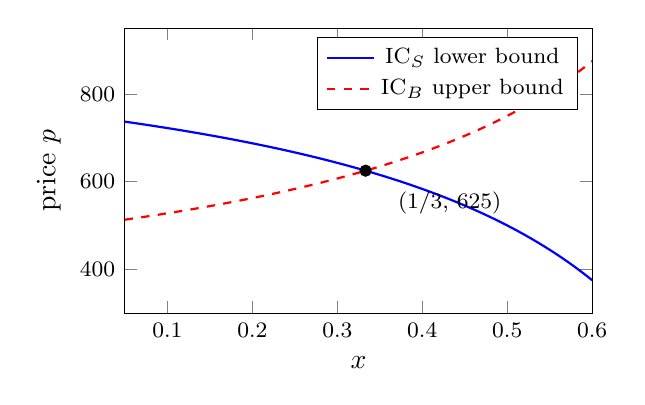
\begin{tikzpicture}
\begin{axis}[width=0.62\textwidth,height=5.2cm,xmin=0.05,xmax=0.6,ymin=300,ymax=950,
  xlabel={$x$},ylabel={price $p$},legend pos=north east,legend style={font=\footnotesize},
  tick label style={font=\footnotesize}]
\addplot[domain=0.05:0.6,samples=80,thick,blue] {750-250*x/(1-x)};
\addlegendentry{IC$_S$ lower bound}
\addplot[domain=0.05:0.6,samples=80,thick,red,dashed] {500+250*x/(1-x)};
\addlegendentry{IC$_B$ upper bound}
\addplot[only marks,mark=*] coordinates {(0.3333,625)};
\node[anchor=north west,font=\footnotesize] at (axis cs:0.36,600) {$(1/3,\,625)$};
\end{axis}
\end{tikzpicture}

{\footnotesize Honest prices exist to the right of $x = 1/3$, where the lower bound lies below
the upper bound.}
\end{center}

\textbf{(f) Why a lower $x$ helps efficiency but defeats it.} A lower $x$ makes the
no-gain pair rarer, so trade is efficient more often ($1-x^2$ rises). But the same $x$ is the
probability that a lie \emph{costs} the liar a trade: a \$1{,}000 buyer who claims \$500 loses the
sale only if the seller is worth \$750 (probability $x$), and a \$250 seller who claims \$750
loses it only if the buyer is worth \$500 (probability $x$). The \emph{gain} from lying is a
better price in the likely cell, which occurs with probability $1-x$. As $x$ falls, lying becomes
almost free, so the rent each tempted type must be promised for honesty approaches the
full \$500 it could grab by lying. Both rents must be paid out of the \$750 surplus of the
(\$250, \$1{,}000) cell: $(p-250) + (1000-p) = 750 \ge 2(500 - k)$, which is exactly $x \ge 1/3$.
Below that there is ``simply not enough surplus to go around'' (\MR, p.~141). A mediator who
maximizes expected gains must then sacrifice some efficient trades, e.g.\ by trading with
probability below one in the cells the liars rely on, which is the incentive-efficiency logic of
\MR{} pp.~143--145.

\interp This is \MR's Table 5.2--5.3 example in disguise: rescaling values by
$(\text{value} - 250)/250$ turns \$250/\$750 and \$500/\$1{,}000 into \$0/\$2 and \$1/\$3. Private
information is a source of inefficiency that no amount of goodwill removes: the feasible set
shrinks once honest reporting must be paid for with informational rents (\MR{} n.~7, p.~141).
Efficient bargaining is easiest precisely when each side's lie is likely to kill a deal, that is,
when the opponent is probably a type with whom a misreport destroys the trade.

\verify Under the rescaling above, $x = 0.2$ reproduces \MR's bounds: $250 + 250 \times 1.75 =
687.5$ and $250 + 250 \times 1.25 = 562.5$, as in the table; $x = 0.8$ is \MR's reversed case,
and their price $p = 1.50$ maps to \$625, inside $[250, 1000]$. \texttt{check\_D.py} solves
IC$_S$ and IC$_B$ symbolically, finds $x^* = 1/3$ and $p = 625$, recomputes every row of the
table and checks that the low types' constraints are implied.

\answer{Trade is efficient except when the buyer is worth \$500 and the seller \$750, so with
probability $1-x^2$. With prices \$500 and \$750 in the other cells, honesty requires
$p \ge 750 - 250x/(1-x)$ (seller) and $p \le 500 + 250x/(1-x)$ (buyer). Both bind at
$x = 1/3$, $p = \$625$. For $x < 1/3$ trade is more often efficient, but lies are almost costless,
the rents needed for honesty exceed the \$750 surplus, and efficient trade is unattainable.}
\end{exsol}
